\documentclass[11pt]{article}
\usepackage[utf8]{inputenc}	% Para caracteres en español
\usepackage{amsmath,amsthm,amsfonts,amssymb,amscd}
\usepackage{multirow,booktabs}
\usepackage[table]{xcolor}
\usepackage{fullpage}
\usepackage{lastpage}
\usepackage{enumitem}
\usepackage{fancyhdr}
\usepackage{mathrsfs}
\usepackage{wrapfig}
\usepackage{setspace}
\usepackage{calc}
\usepackage{multicol}
\usepackage{cancel}
\usepackage[retainorgcmds]{IEEEtrantools}
\usepackage[margin=2cm]{geometry}
\usepackage{amsmath}
\newlength{\tabcont}
\setlength{\parindent}{0.0in}
\setlength{\parskip}{0.05in}
\usepackage{empheq}
\usepackage{framed}
\usepackage[most]{tcolorbox}
\usepackage{listings}
\usepackage{xcolor}
\usepackage{tikz}
\usepackage{pgfplots}
\pgfplotsset{compat=newest}
\colorlet{shadecolor}{orange!15}
\parindent 0in
\parskip 12pt
\geometry{margin=0.5in, headsep=0.25in}
\theoremstyle{definition}
\newtheorem{defn}{Definition}
\newtheorem{reg}{Rule}
\newtheorem{exer}{Exercise}
\newtheorem{note}{Note}
\begin{document}
\newcommand{\bvec}{\mathbf}
\newcommand*\Dcancelto[2][0]{%
  \kern9pt%
  \begin{tikzpicture}[baseline=(current bounding box.center).anchor=west]
    \node[anchor=east,inner sep=2pt] (a) {#2};
    \draw[->] ($(a.north west)+(1pt,-2pt)$) -- ($(a.south east)+(0pt,2pt)$) node at ($(a.south east)+(4pt,1pt)$) {$\canc{#1}$};
\end{tikzpicture}
}

\definecolor{codegreen}{rgb}{0,0.6,0}
\definecolor{codegray}{rgb}{0.5,0.5,0.5}
\definecolor{codepurple}{rgb}{0.58,0,0.82}
\definecolor{backcolour}{rgb}{0.95,0.95,0.92}

\lstdefinestyle{mystyle}{
    backgroundcolor=\color{backcolour},   
    commentstyle=\color{codegreen},
    keywordstyle=\color{magenta},
    numberstyle=\tiny\color{codegray},
    stringstyle=\color{codepurple},
    basicstyle=\ttfamily\footnotesize,
    breakatwhitespace=false,         
    breaklines=true,                 
    captionpos=b,                    
    keepspaces=true,                 
    numbers=left,                    
    numbersep=5pt,                  
    showspaces=false,                
    showstringspaces=false,
    showtabs=false,                  
    tabsize=2
}

\lstset{style=mystyle}




\title{
    \begin{center}
        \textbf{m-dimentional Multinomial statistical model}
    \end{center}
    \begin{center}
        \textbf{Programming Exercise 4}
    \end{center}
\large MAP2212 - 2023/1
}
\author{Julian Sousa - 11846922}
\date{}
\maketitle
\section{Introdução}
O objetivo deste trabalho era desenvolver um modelo de deep learning capaz de classificar estrelas com base no diagrama H-R. Foi abordado o problema da classificação de estrelas com base nas características de temperatura, luminosidade, raio e magnitude absoluta presentes no diagrama Hertzsprung-Russell (H-R). As estrelas foram categorizadas em diferentes tipos e estágios evolutivos, incluindo Anã Marrom, Anã Vermelha, Anã Branca, Sequência Principal, Supergigante e Hipergigante.

O diagrama H-R é uma representação gráfica que mostra a relação entre a luminosidade (magnitude absoluta) e a temperatura (cor) das estrelas. A classificação precisa das estrelas com base nesse diagrama pode fornecer insights valiosos sobre sua evolução, estrutura e propriedades físicas. Além disso, a capacidade de automatizar esse processo de classificação pode economizar tempo e esforço dos astrônomos.

Neste trabalho, será descrito o tratamento dos dados, incluindo a preparação dos dados, a normalização e o particionamento em conjuntos de treinamento e teste. Em seguida, será apresentado o modelo de deep learning utilizado, sua arquitetura e os parâmetros de treinamento. Por fim, serão analisados os resultados obtidos e serão discutidas as conclusões e possíveis melhorias

\pagebreak
\section*{Inspeção dos dados}
Plotando os dados de acordo com a magnitude absoluta e temperatura, foi obtido o seguinte resultado:
\begin{figure}[htbp]
    \begin{center}
        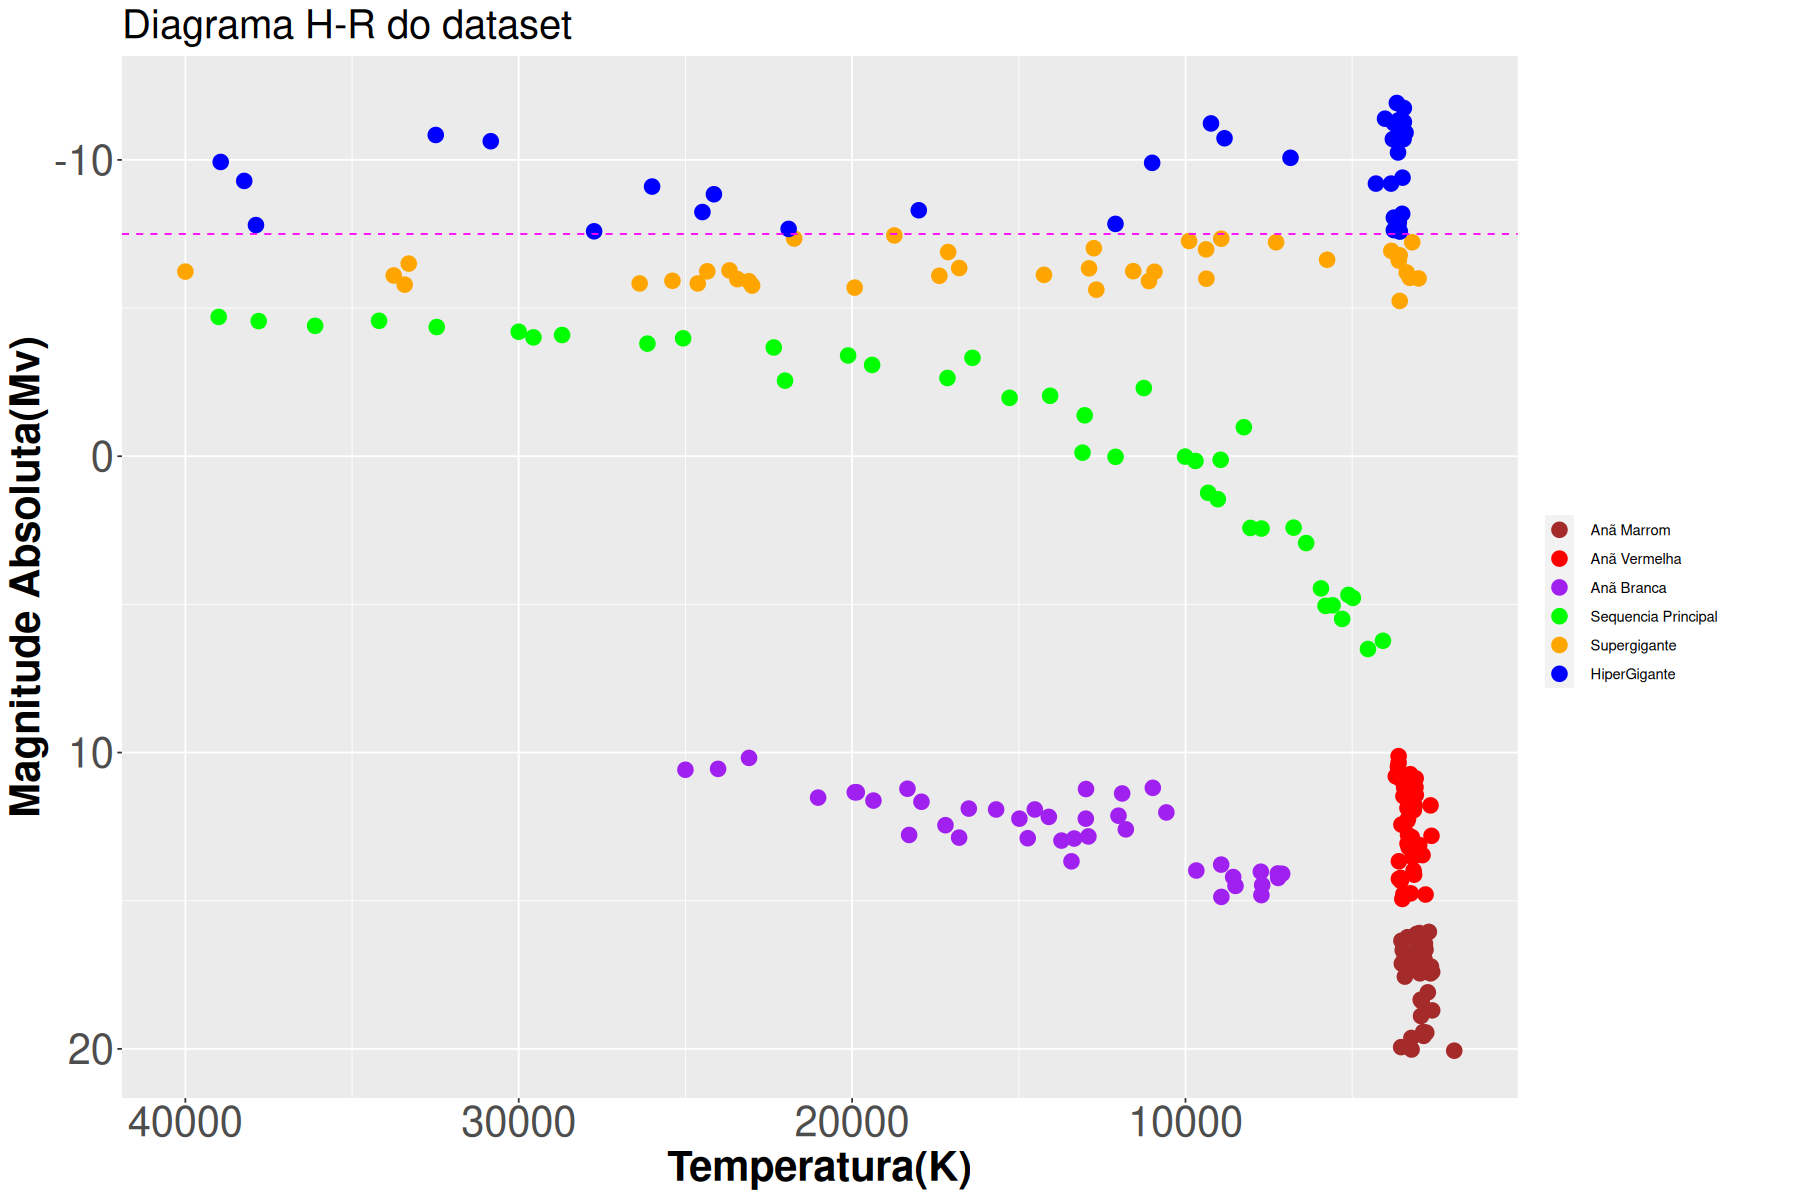
\includegraphics[scale=0.5]{../plot_hr_full.png}
    \end{center}
\end{figure}

que está de acordo com o modelo H-R padrão.



\section{Preprocessamento e Exploração}

Para o tratamento dos dados, foram seguidos os seguintes passos:

\subsection{Remoção das features textuais}
Inicialmente, foram removidas as features textuais, ou seja, as colunas que continham informações de cor e classe espectral. Essas features não são diretamente utilizáveis em modelos de machine learning, e o foco era a modelagem com base nas features numéricas restantes.

\subsection{Normalização das features numéricas}
Após a remoção das features textuais, as features numéricas restantes foram normalizadas. A normalização é um processo importante para garantir que todas as features tenham a mesma escala e não dominem o modelo devido a diferenças nas unidades ou faixas de valores. Isso ajuda a evitar vieses indesejados e melhora a estabilidade e a convergência do modelo durante o treinamento.

\subsection{Inspeção da matriz de correlação}
A matriz de correlação foi calculada entre as features numéricas remanescentes. Essa análise permitiu avaliar a relação linear entre as variáveis e identificar possíveis padrões ou dependências entre elas. A visualização da matriz de correlação auxilia na compreensão das relações entre as features e pode ajudar a identificar features redundantes ou altamente correlacionadas, que podem ser removidas para evitar multicolinearidade.
\begin{figure}[htbp]
    \begin{center}
        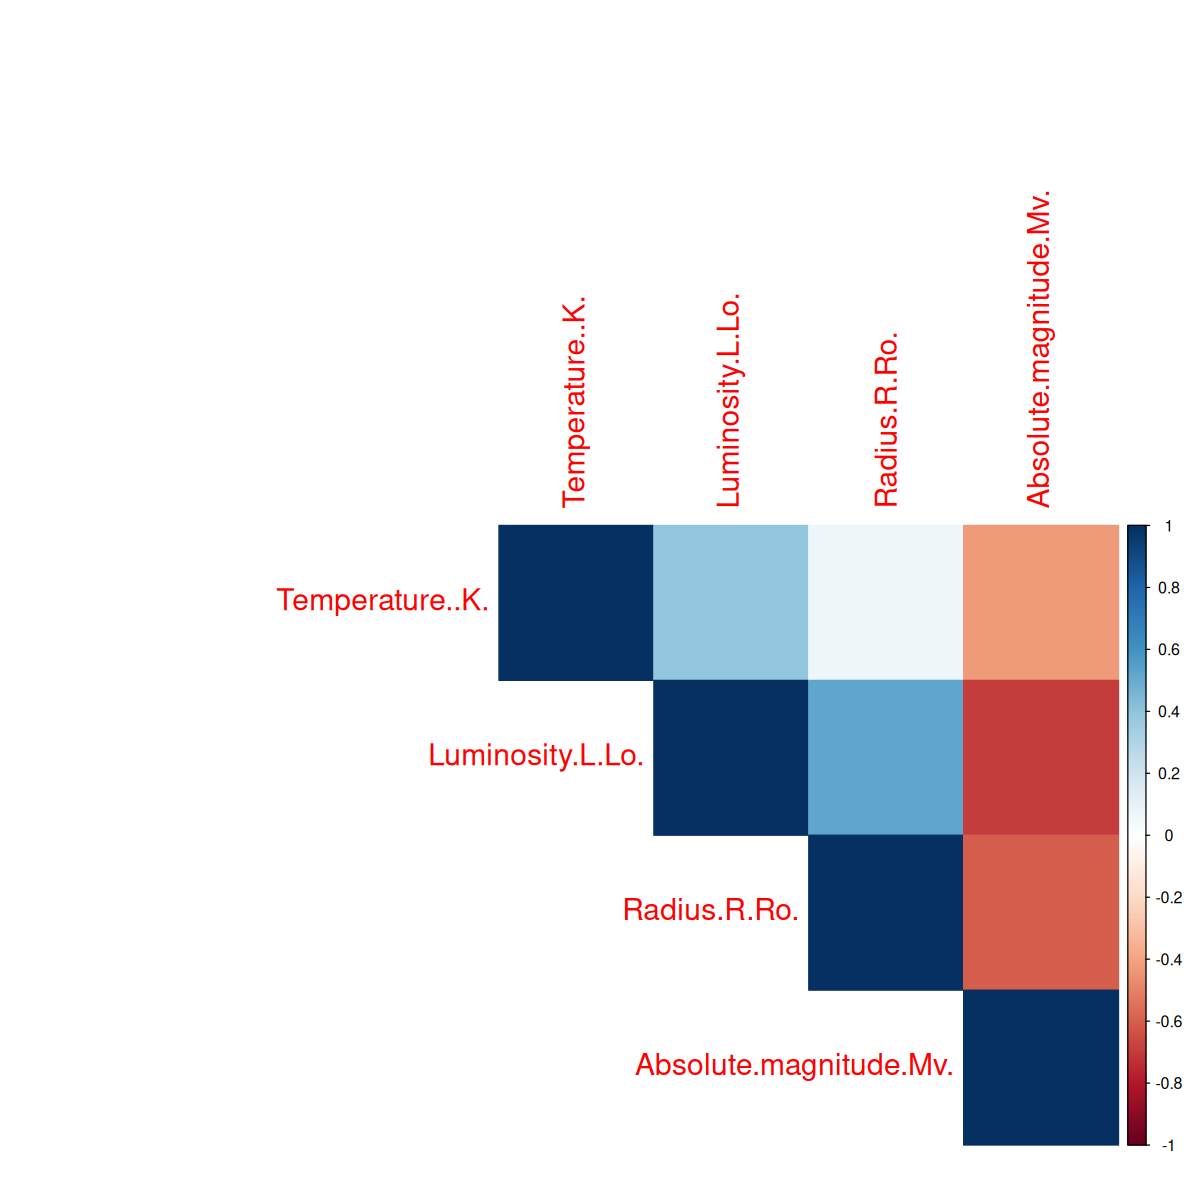
\includegraphics[scale=0.5]{../correlation_matrix.png}
    \end{center}
\end{figure}

Como podemos observar, existem relações relevantes de correlação entre as características das estrelas,
portanto, podemos levantar a hipótese de que um modelo de classificação possa tirar conclusões sobre a natureza das mesmas, com base na análise destas features.

Além disso é podemos observar que a magnitude absoluta de uma estrela, é inversamente proporcional a todas as outras
características estudadas, em particular, vale notar a forte correlação (approx -0.8) entre Luminosidade e Magnitude, o
que indica que estas colunas podem apresentar forte influencia na decisão final do modelo treinado.

\subsection{Separação em conjunto de treino e teste}
Após o tratamento dos dados, os conjuntos de treino e teste foram criados. A separação dos dados em conjuntos de treinamento e teste é essencial para avaliar o desempenho do modelo em dados não vistos previamente. Geralmente, uma porcentagem dos dados é reservada para o conjunto de teste, enquanto o restante é utilizado para treinar o modelo. Essa divisão permite medir a capacidade de generalização do modelo e identificar possíveis problemas de overfitting ou underfitting.

Ao seguir esses passos, os dados foram preparados e prontos para serem utilizados no treinamento e avaliação do modelo de classificação de estrelas com base no diagrama H-R.

\section{Modelo de Ajuste}

O modelo utilizado para ajustar os dados foi uma rede neural do tipo sequencial, construída com o pacote Keras. O modelo foi definido com as seguintes camadas:

\begin{verbatim}
model <- keras_model_sequential()
model %>%
  layer_flatten(input_shape = c(4)) %>%
  layer_dense(units = 200, activation = "relu") %>%
  layer_dense(units = 6, activation = "softmax")
\end{verbatim}

O modelo consiste nas seguintes camadas:

\begin{itemize}
  \item Camada de Achatamento (\textit{Flatten}): Essa camada recebe os dados de entrada com 4 features e os transforma em um vetor unidimensional. Isso permite que as features sejam processadas pelas camadas subsequentes da rede neural.
  \item Camada Densa (\textit{Dense}): Essa camada possui 200 unidades (neurônios) e utiliza a função de ativação ReLU. A camada densa é responsável por realizar a computação de transformações lineares e não lineares nos dados de entrada.
  \item Camada Densa de Saída: Essa camada possui 6 unidades e utiliza a função de ativação \textit{softmax}. A camada de saída produzirá uma distribuição de probabilidade sobre as 6 classes de estrelas possíveis.
\end{itemize}

O modelo foi compilado com os seguintes parâmetros:

\begin{verbatim}
model %>% compile(
  optimizer = "adam",
  loss = "sparse_categorical_crossentropy",
  metrics = c("accuracy")
)
\end{verbatim}

\begin{itemize}
  \item Otimizador: Foi utilizado o otimizador Adam, que é uma técnica de otimização baseada em descida de gradiente estocástica. O otimizador é responsável por ajustar os pesos da rede neural durante o treinamento.
  \item Função de Perda: Foi utilizada a função de perda \textit{sparse categorical crossentropy}. Essa função é apropriada para problemas de classificação com várias classes e trata as classes como mutuamente exclusivas.
  \item Métricas: A métrica de avaliação utilizada foi a acurácia (\textit{accuracy}), que mede a proporção de previsões corretas em relação ao total de previsões.
\end{itemize}

\section{}






\end{document}

